Time-series prediction of neural models rely on an input history of equally distributed samples.
\ifthenelse {\boolean{thesis}}{As discussed in earlier chapters, the LSTM model is a recurrent neural network designed to solve the vanishing gradient problem by remembering (preserving) the long dependencies \cite{rasifaghihi_predictive_2020}.}
{The LSTM model is a recurrent neural network designed to solve the vanishing gradient problem by remembering (preserving) the long dependencies~\cite{rasifaghihi_predictive_2020}.}
The cells inside the model act as memory units to preserve the dependence.
Therefore, the output is closely dependent on the previous input samples.
Unlike the normal RNN and the more modern version GRU, LSTM has a more complicated structure constructed from several logical gates~\cite{LSTM_Hochreiter1997}.
% It is the most widely used type of model.
\ifthenelse {\boolean{thesis}}{Chapter~\ref{cha:Analysis} provides a summary of the LSTM cell logic, with corresponding equations explaining the gates logic in detail.} 
{}
% \mbox{Figure~\ref{fig:LSTM-cell2}} provides a summary of the cell logic.
% The decisions are based around sigmoid $\sigma$ equation~\ref{eq:sigmoid2}.
% \begin{equation}
%     \sigma(x) = \frac{1}{1+e^{-x}}
%     \label{eq:sigmoid2}
% \end{equation}
% The cell logic utilises three gates.
% Forget $f_t$ to control the level of information to ignore, input $i_t$ to decide upon relevant information to add and output $o_t$ to determine the influence to model at the current step, \mbox{equation~\ref{eq:LSTM-gates2}}.
% \begin{equation}
%     \begin{split}
%         f_t &= \sigma \left(W_f \left[h_{t-1}, x_t \right] + b_f \right) \\
%         i_t &= \sigma \left(W_i \left[h_{t-1}, x_t \right] + b_i \right) \\
%         o_t &= \sigma \left(W_o \left[h_{t-1}, x_t \right] + b_o \right) \\    
%     \end{split}
%     \label{eq:LSTM-gates2}
% \end{equation}
% The $tanh$ activation function is used as the default in procedures for cell state update and further propagation, \mbox{equation~\ref{eq:LSTM-output2}}.
% Variables $h_t$ and $c_t$ represent memory cell output and the cell state at timestamp $t$.
% \begin{equation}
%     \begin{split}
%         c_t &= f_t c_{t-1}+i_t \times tanh \left(W_c \left[h_{t-1}, x_t \right] + b_c \right) \\
%         h_t &= o_t*tanh \left(c_t \right)
%     \end{split}
%     \label{eq:LSTM-output2}
% \end{equation}
% \begin{figure}[htbp]
%     \centering
%     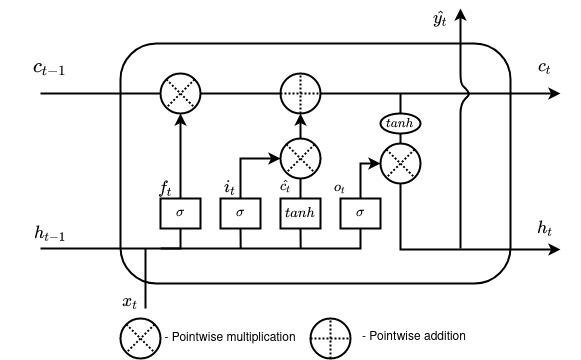
\includegraphics[width=0.8\columnwidth]{II_Body/LSTM/images/LSTM.jpg}
%     \caption{Long Short-Term Memory Cell}
%     \label{fig:LSTM-cell2}
% \end{figure}
% }
%
%
%? May 19 2023 - removing paragraph from article.
\ifthenelse {\boolean{thesis}}{The LSTM model has been used widely in stock price prediction or weather forecasting. 
%? add references if I feel to it
However, unlike State of Charge estimation, which commonly uses $V$, $I$, and $T$ as inputs, those methods utilise the output feature as an input to the subsequent prediction to propagate results further and calculate the time before a critical event occurrence.
Besides, methods like weather forecasting for a week are not limited by lacking output data since the searched criteria are always known or will be known once they happen, allowing updates and improvements of follow-up predictions.
Contrary to this case, a battery's actual State of Charge cannot be directly determined or measured, making verification against previously-made predictions difficult without additional battery modelling techniques or laboratory equipment.
%, not to mention having it integrated into an Electric Vehicle's accumulator.
It can be determined with a proper battery cycler, performing a set of pulse tests, which is infeasible for practical EV applications.
%utilising a battery and affecting its charge and remaining life.
% (As opposed to the SoC estimate, where getting actual values to require a battery cycler capable ... ) 
%%%%%%%%%%%
%Unlike the charge estimation, which can only output a single value based on a history of samples, they are not limited to ... . Therefore, it does not require the output as input since the truth will become known in due time.
As such, to include the charge in the process, SoC as a learning input is used, later making a predicted array of values used on testing.
Such an approach introduces potential issues for error accumulation with every evaluation that will be addressed.
} {} 

%
%
The best way to use the performance of the stateless LSTM model is through training with a data windowing technique.
The NN model will receive a fixed set of equally-distributed time samples at each time prediction.
Every next forecast will shift the time window by a constant step $s$, until all possible combinations of time slices have gone through the training model.
That approach is called a stateless model, which only sees dependencies over the input sample range, rather than preserving every received input, like in stateful implementations.
It also allows the order of the windows to be shuffled to avoid overfitting.
% Since no \textit{Dropout} layer was applied before the model's output, a set of strategies has been applied to update the learning rate and rollback before early stopping to assist the fitting process.
To produce repeatable and comparable results and assist the fitting process, the \textit{Droput} layer, to avoid overfitting at the end of the layer, has been replaced with strategies that update the learning rate and rollback before early stopping.
\ifthenelse {\boolean{thesis}}{Chapter~\ref{cha:Analysis} at subsections~\ref{subsec:l-rate} and~\ref{subsec:t_model} explain those two methods, which have already proven to be effective at training SoC models.} 
{Early research on published methods has already utilised those two methods to assist the models' training process~\cite{sadykov_practical_2022}.
It involved a scheduled learning rate value update with every passing epoch for as long as the accuracy kept improving with every passing iteration, as well as assisting the models' recovery in the event of overfitting by double reduction of the rate either until the models' return to the same minimal fitting or finalises the optimum result reach.}
As a result, a NN model will learn dependency between a fixed amount of equally distributed time samples $n$ and yet be independent of the order of the inputs.
\ifthenelse {\boolean{thesis}}{\mbox{Figure~\ref{fig:Windowing}} adapts the earlier Figure~\ref{fig:Windowing3f}, demonstrating how the input dataset is constructed and ordered into a 3-dimensional dataset, with four features (Voltage, Current, Temperature and added initial SoC), 500 timestamps and around a hundred thousand samples to fit on.}{}

%
%
\textcolor{blue}{Here, in Figure~\ref{fig:windowing_simple}, a time-series training set of equally spaced data points is broken up into "windows" of a set width (5 samples in this case), with a difference by one sample from the previous one by \textit{s}-step.
A window is defined starting at each data point so that each window overlaps with the next windows, shifted by \textit{s} number of samples.}
Each window is associated with an output parameter.
The process can be broadly explained in simple terms whereby, prediction using a trained LSTM model of this type will take a window width of input samples and then effectively "choose" the window of best fit from the trained data set, outputting the associated parameter, much like how image recognition works.
\begin{figure}[hbp]
    \centering
    % DST based tests 0.8
    \includesvg[width=\columnwidth]{II_Body/images/simple_windows.svg}
    \caption{Simple windowing example.}
    \label{fig:windowing_simple}
\end{figure}
\begin{landscape}
    \begin{figure}[t]
        \centering
        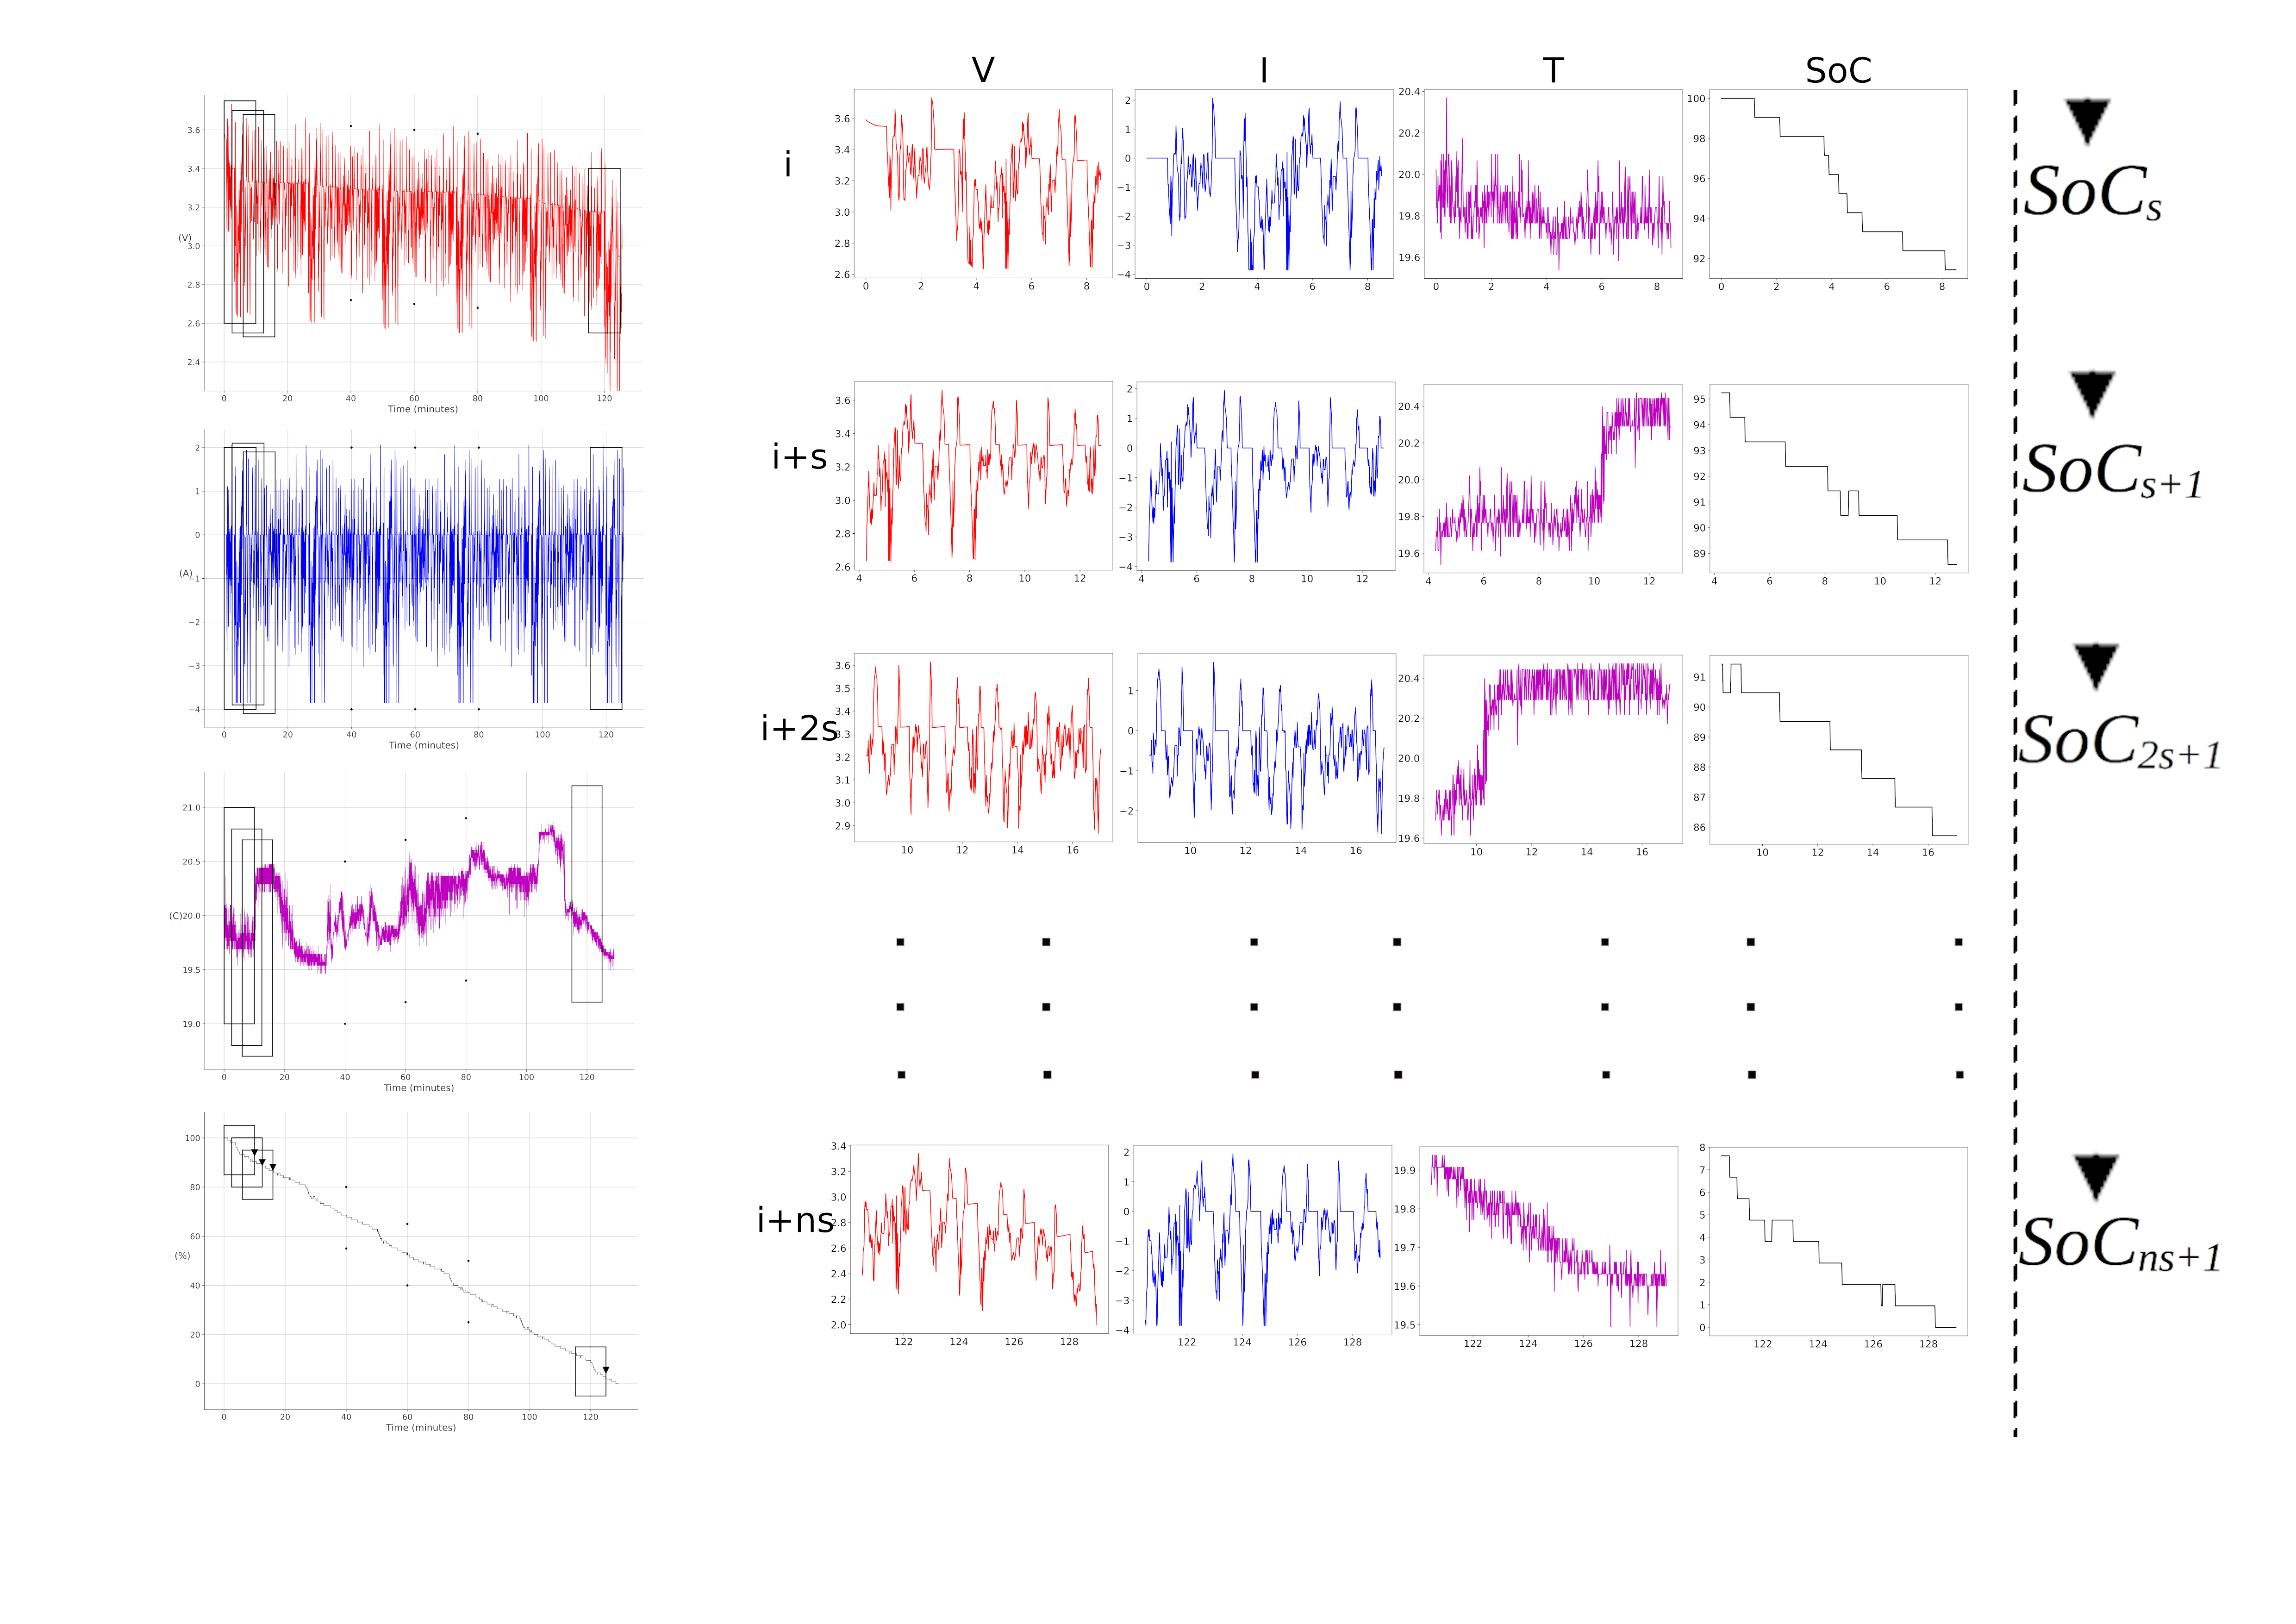
\includegraphics[width=\linewidth]{II_Body/images/Windowing4f-A3.jpg}
        \caption{Data Windowing scheme at 1Hz sampling rate. For visualisation purposes, the $s$-skip has been used as 250 seconds, which is different from the actual implementation. The initial index $i$ was kept as a value close to the beginning of the data, around zero, excluding possible initial data discrepancies.}
        \label{fig:Windowing}
    \end{figure}
\end{landscape}
\mbox{Figure~\ref{fig:Windowing}} demonstrates how those windows in the dataset are constructed and ordered into a 3-dimensional data, with four features, 500 timestamps and around a hundred thousand samples to fit on.
Due to the size of the windows, equivalent to 8 and a quarter minutes of a discharge process, \textcolor{blue}{with only 1 sample shift \textit{s} between each other}, no batching mechanism has been used to reduce computational load and avoid 4-dimensional matrix management.
In this work, the data set has four features, namely current, voltage, temperature and SoC, and an output parameter of a single SoC value (i.e the next SoC immediately following the window set.)
% The full windowing classification of this data is represented in Figure 2.
For such multi-dimensional arrays, the training/prediction can happen in any order, since the model gets all required information to train and adjust weights within a windows of inputs and associated outputs.
% The same has been true for previous research in this area~\cite{sadykov_practical_2022}, but will be explored further, by building up on the derived conclusions and introducing a sequential way of testing model in Feed-Forward manner, similar to the behaviour of the real driving conditions.}

%
%
\ifthenelse {\boolean{thesis}}{Similar to Chapter~\ref{cha:Analysis}, to speed up the training process, the mean and standard deviation of each of the four features has been used to normalise all data.}
{To speed up the training process, the mean and standard deviation of each of the four features has been used to normalise all data.}
The normalisation constant from training input samples has been used for all further validation and testing sets to ensure the right trends.
To simplify the implementation of SoC being both an input and output feature and fit to real-world scenario inside a battery pack, it has been narrowed between 0 and 1 to represent the percentage charge to two decimals and shifted by one sample back to associate Voltage, Current and Temperature with an existing SoC value, not the one which will be theoretically predicted; referred to as \textit{previous} or \textit{known} SoC in the remainder of this work.
\mbox{Table~\ref{tab:params}} highlights the parameters required to define the initial model, where $AR$ defines output step size, which will be justified later in Section~\ref{sec:feed}.
A $\sigma$ function as an output justifies the charge normalisation between 0 and 1.
\ifthenelse {\boolean{thesis}}{The number of neurons has been selected based on the results made in Chapter~\ref{cha:Analysis}, Section~\ref{sec:AN:Results}.
Even though the number of neurons was kept as per the performance result table, only one layer has been utilised due to manual implementation of the model and the inability to validate the multilayer implementation correctness against some published or already-used models.
It was decided to stick to known approaches to validate the efficiency of the newly-proposed technique.
\begin{table}[ht]
    \renewcommand{\arraystretch}{1.3}
    \caption{Model structure and parameters}
    \centering
    \label{tab:params}
    \begin{tabular}{ l l l }
        \hline\hline \\[-4mm]
        Input     & $shape= \left( 1,500,4 \right)$ & $batch=1 $  \\
        \hline
        LSTM      & $activation=tanh$ & $units=131$  \\
        \hline
        Dropout   & $0.0$ &   \\
        \hline
        Output    & $activation= \sigma\left(s, 1 \right)$ &   \\
        \hline\hline
    \end{tabular}
\end{table}
}
{The number of neurons has been selected based on the results made on earlier discoveries of the most optimal hyperparameters set~\cite{sadykov_practical_2022}.
\textcolor{blue}{Only a single layer RNN will be utilised throughout the work due to the primary focus on the Autoregression method that requires proper testing before further improvements.
Therefore, an effective combination of layers and neurons will be outside of the scope and will only be based on the results discovered early.
The results section was adapted} to the new custom-implemented model to validate the technique's efficiency in a comparable way with already-tested approaches.
\begin{table}[ht]
    \renewcommand{\arraystretch}{1.3}
    \caption{Model structure and parameters}
    \centering
    \label{tab:params}
    \resizebox{\columnwidth}{!}{
    \begin{tabular}{ l l l }
        \hline\hline \\[-4mm]
        Input     & $shape= \left( 1,500,4 \right)$ & $batch=1 $  \\
        \hline
        LSTM      & $activation=tanh$ & $units=131$  \\
        \hline
        Dropout   & $0.0$ &   \\
        \hline
        Output    & $activation= \sigma\left(AR, 1 \right)$ &   \\
        \hline\hline
    \end{tabular}
    }
\end{table}
}

%
%
\ifthenelse {\boolean{thesis}}
{
The optimisation algorithm for the fitting process have been selected as the regular Adam method, which was highlighted in Chapter~\ref{cha:Analysis}, \mbox{Algorithm~\ref{alg:Adam}}, with the corresponding hyperparameters, \mbox{Table~\ref{tab:uni-hyperparams}}.
The selection of this optimiser is made to allow comparison to two early-created LSTM-based models which use the same optimiser in Chapter~\ref{cha:Analysis}.
}
{
The optimisation algorithm for the fitting process has been defined by Adam, \mbox{Algorithm~\ref{alg:copyAdam}}, with the corresponding inputs changes and hyperparameters on \mbox{Table~\ref{tab:newM-params}}. %? Return Adam paper reference if space would allow
%\textcolor{red}{Try to use Robust Adam instead, because why the hell not since I lost one month of my life to implement that cursed algorithm from Javids miss-typed notes? Complete this section with details as per Gareth Javid's implementation if RoAdam will be able to produce a faster fitting.}
\begin{algorithm}\captionsetup{labelfont={sc,bf}, labelsep=newline}
    \caption{Adaptive Moment Estimation (Adam) optimisation}
    \begin{algorithmic}[1]
        \STATE \textbf{Number of input samples} \\ $N\gets length(\textit{input data})$\\
        \STATE \textbf{Size of windows} \\ $S\gets length(V_{i..n})$\\
        \STATE \textbf{Output steps} \\ $O\gets length(V_{i..n})$\\
        \STATE Input: $x_n = [V_{i..n}, I_{i..n}, T_{i..n}, SoC_{(i-1)..(n-1))}]$ \\
        - Shape: $X = (N, S, 4)$
        \STATE Output:$y_n = [SoC_{(n-o)..n}] - $Shape:$Y = (N, O, 1)$
        \STATE Define Loss function: $L$ \\
                Get hyperparameters: $\alpha, \beta_1, \beta_2, \epsilon$
        \WHILE{$W_t \text{ does not converge}$}
        \STATE $t \gets t+1$
        \STATE $g_t \gets \nabla_W L_t (W_{t-1})$ \COMMENT{Obtain gradient}
        \STATE $m_t \gets \beta_1 m_{t-1}+(1-\beta_1) g_t $ \COMMENT{$1_{st}$ moment calculation}
        \STATE $\upsilon_t \gets \beta_2 \upsilon_{t-1}+ \left(1-\beta_2 \right)g^2_t $ \COMMENT{$2_{nd}$ moment calculation \label{alg:Adam-Line-2Moment}}
        \STATE $\hat{m_t} \gets \frac{m_t}{1-\beta^t_1}$ \COMMENT{Corrected $\hat{m_t}$}
        \STATE $\hat{\upsilon_t} \gets \frac{\upsilon_t}{1-\beta^t_2} $ \COMMENT{Corrected $\hat{\upsilon_t}$}
        \STATE $W_t \gets W_{t-1}- \alpha \frac{\hat{m_t}}{\sqrt{\hat{\upsilon_t}}+\epsilon} $ \COMMENT{Update parameters}
        \ENDWHILE
    \end{algorithmic}
    \label{alg:copyAdam}
\end{algorithm}
\begin{table}[htbp]
    \renewcommand{\arraystretch}{1.3}
    \caption{Optimiser Hyper-Parameters}
    \centering
    \label{tab:newM-params}
    \resizebox{\columnwidth}{!}{
    \begin{tabular}{ l l l l l l }
        \hline\hline \\[-3mm]
        $\alpha$ & $\beta_1 $ & $\beta_2$ & $\beta_3$ &  $\epsilon$ \\
        \hline
        Linear         &  &  &  & \\% 0.0000001
        Scheduler      & $0.9$ & $0.999$ & $0.999$ &$10^{-8}$ \\% 0.0000001
        (0.001-0.0001) &  &  &  & \\% 0.0000001
        \hline\hline
    \end{tabular}
    }
\end{table}
}